\section*{Data Sets}
	%subsection{Description}	
	Our network data set has been accumulated with a lot of effort over the years and hyperlinks to most of the data are available at the website of The Colorado Index of Complex Networks (ICON) \url{https://icon.colorado.edu}. ICON is a place where hyperlinks to the network data are stored, rather than the data itself.  
	Since the data format of real world networks is not standardized, we proceeded to convert all the data into a single format called \textit{Graph Modeling Language} or simply GML \cite{GML}. The format allows us to flexibly specify arbitrary node and edge attributes. We, however, do not use any node and edge attribute, including edge weight, as well as edge directionality at all since not all networks have such properties and we wanted to analyze a diverse set of networks. Thus, we treat all networks used in this study as a simple graph which is defined in the previous section. We have used only a fraction of all networks available on ICON due to the time constraint. We have also added some synthesized network data which are generated from four specific models briefly explained in the following:
	 
	\begin{enumerate}
		\item Erd\H{o}s-R\'enyi random network model (ER Network) \cite{ER_Network}, where given $n$ the number of edges and $p$ the probability that a pair of nodes gets connected, for each pair of nodes in the network, one connects the nodes according to $p$. This model yields the average path length of $O(\log n)$ and low clustering coefficient.
		
		\item Watts-Strogatz model (Small World) \cite{watts1998cds} which produces a network having the high clustering coefficient and low average path length of $O(\log n)$. The model starts with a grid network and then rewires some edges according to some probability $p$. The rewiring makes the network's path length smaller while keeping the high clustering due to the gird structure.
		
		\item Barab\'asi-Albert model (Scale Free) \cite{Barabasi99emergenceScaling} with which one grows a network over the course of time. Newly added nodes have a fixed number of edges attached to them, and these edges connect to the existing nodes according to the probability $p$ that is proportional to the degree of an existing node. Therefore nodes having many connections will be more likely to receive more edges attached to them. Although this model was originally invented by Price in a paper in 1965 \cite{deSollaPrice1965}, we call the model as BA model since it's more widely known as its name.
		
		\item The Forest Fire network model (Forest Fire Network) \cite{ForestFire} which is a network generative model with the following procedures: (i) a newly added node $u$ attaches to (cites) some existing nodes, called \textit{ambassadors}, chosen uniformly at random; (ii) for each newly cited node $v$, its incoming and out-going neighbors are also cited by $u$, the new node; (iii) the same procedure is done recursively for all of the newly cited nodes.
	\end{enumerate}

We show all the details of network sub-domains for our study in the Table \ref{tab:subdomain}. The distributions of network domains and sub-domains, as shown in Figs.~\ref{domain_ratio} and \ref{sub_dist}, are very skewed since instances of some network categories are hard to obtain due to their inherent difficulty of collecting data or legal concerns, or hard to analyze due to their network size and this leads us to explore several sampling methods, which are explained in the following section. 
	
%\subsection{Feature Extraction}
After converting into GML format, we calculate a set of features explained in the previous section for each network. We have extensively used a Python library \textit{igraph} \cite{igraph} for extracting features including clustering coefficient and degree assortativity and other miscellaneous operations on network data. For calculating network motifs, we used a parallel motif computing algorithm for undirected motifs developed by Ahmed \textit{et al.} \cite{ahmed2015icdm}. A number of computations involved in this study are parallelized by using a command-line tool \textit{GNU Parallel} \cite{GNUParallel}.


\begin{figure*}
\centering 
\subfloat[The categorical ratio of network domains]{%
  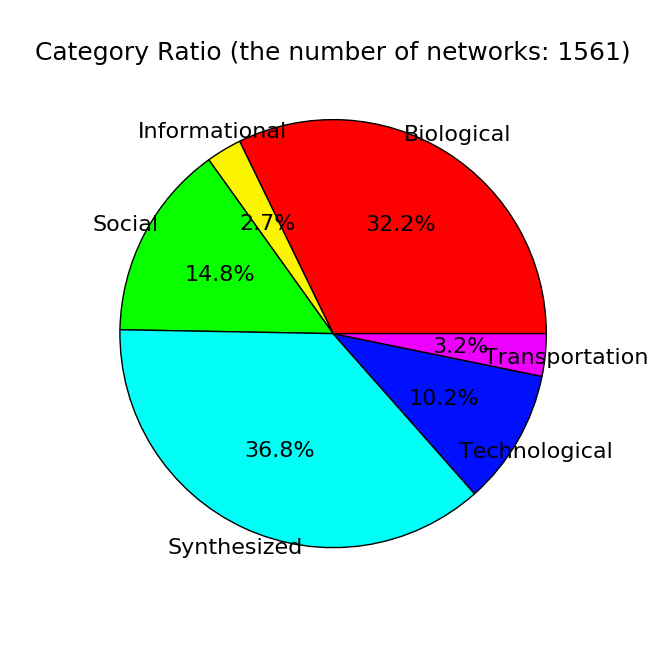
\includegraphics[width=0.85\columnwidth]{figs/category_ratio.png}%
  \label{domain_ratio}%
}\qquad
\subfloat[Count distribution of network sub-domains.]{%
  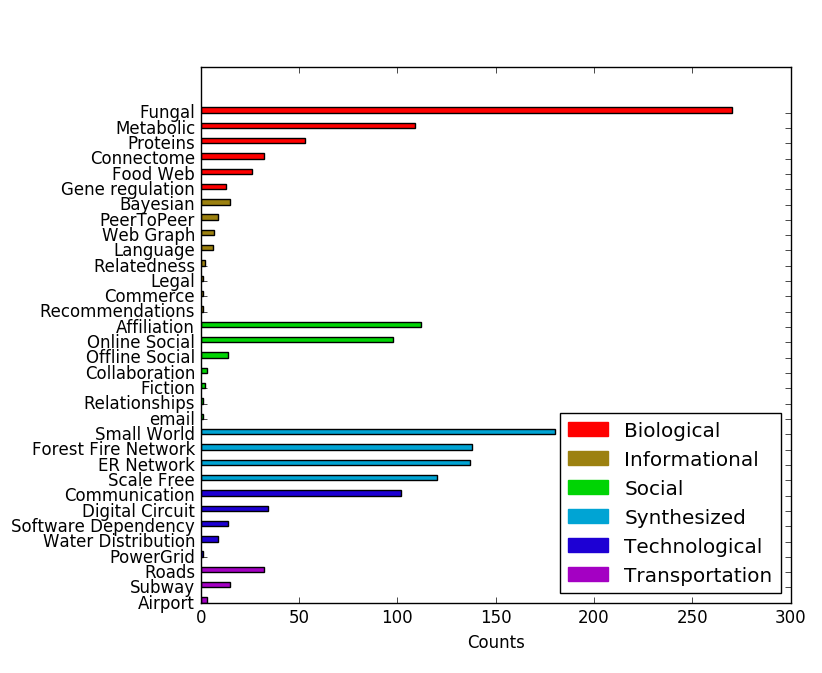
\includegraphics[width=0.85\columnwidth]{figs/subdomain_dist.png}%
  \label{sub_dist}%
}

\caption{ Sub-domains of the same network domain are grouped together having the same color in the figure. Color code from top: Biological, Informational, Social, Synthesized, Technological and Transportation.} \label{category_dist}.

\end{figure*}
